\documentclass[a4paper,openright,10pt]{article}
\usepackage[spanish]{babel} 
\usepackage[utf8]{inputenc}
\usepackage[usenames]{color}
\usepackage[T1]{fontenc}
\usepackage{lmodern}
\usepackage{float}
%Formato figuras
\usepackage{graphicx}
\usepackage{minted}
%Márgenes
\usepackage[left=2.5cm,top=2.5cm,right=2.0cm,bottom=2.5cm]{geometry}
\usepackage[hidelinks]{hyperref} 
\usepackage[usenames]{color}

\graphicspath{{./Figuras/}}



\begin{document}


%PORTADA
\pagestyle{empty} %Quitar el formato predeterminado a la primera hoja
\begin{center}
\vspace*{-1.5cm}
\begin{figure}
\centering
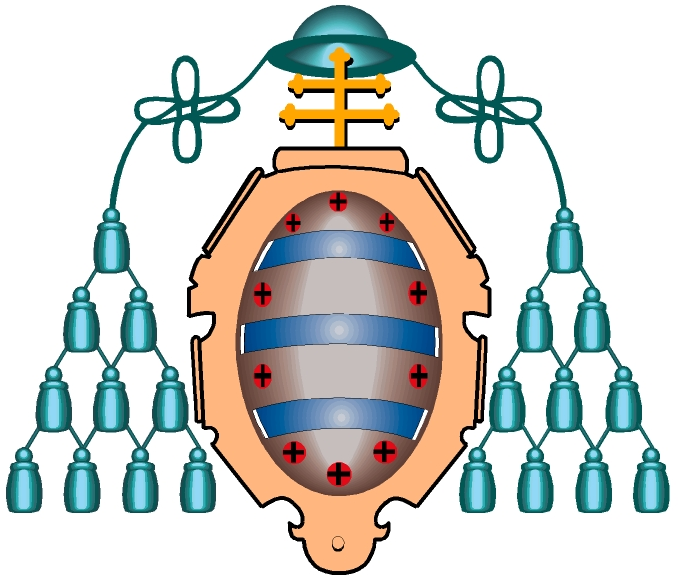
\includegraphics[width=4cm]{uniovi.png}
\end{figure}
\vspace*{0.5cm}
\rule{80mm}{0.1mm}

\begin{Large}

Universidad de Oviedo
	
\end{Large}

Escuela Politécnica de Ingeniería de Gijón

\vspace*{3cm}

\begin{Large}

Grado en Tecnologías y Servicios de la Telecomunicación
	
\end{Large}

\vspace*{0.17cm}

Aplicaciones Telemáticas

\vspace*{1cm}

\begin{huge}

Sesión 1.2 - Especificación, diseño e implementación de un protocolo

\end{huge}

\vspace*{0.5cm}

Marco Martínez Ávila
	
\end{center}

\begin{center}
	
\vspace*{2cm}
\centering

\includegraphics[width=3cm]{logo.png}
	
	
\end{center}

\clearpage

\pagestyle{plain} %Añadir numeración a las páginas siguientes


\section {Descripción de la práctica}

En esta práctica se ampliará la funcionalidad del servicio web implementado, añadiendo la posibilidad de resolver sistemas de ecuaciones de 2 y 3 incógnitas. Además, se consumirá ese servicio desde un cliente Java, utilizando el IDE Eclipse.

\section{Descripción del trabajo realizado}

La inclusión de la nueva funcionalidad, la resolución de sistemas de ecuaciones, tiene su origen en la modificación de la interfaz ``IMath.cs''. Es necesario definir un nuevo \textit{OperationContract} (método), de forma que los clientes puedan utilizarlo para consumir esta nueva opción.

\begin{minted}{csharp}
	[OperationContract]
	double[] SolveSystem(double[] system);
\end{minted}

La implementación de la funcionalidad necesaria se realiza por medio de la biblioteca ``EcSystem''. No se encontró ninguna biblioteca externa que permitiera añadir esta opción de forma directa, por lo que se optó por modificar un fragmento de código que permitía resolver ecuaciones utilizando el método de Cramer para adaptarlo a los requerimientos de esta práctica.

Se decidió que el argumento que recibe la función ``SolveSystem'' sea un array de \textit{double}, conteniendo los valores del sistema de ecuaciones sin resolver. A su vez, el método devolverá otro array del mismo tipo, conteniendo los valores para las variables que correspondan.

Posteriormente, y una vez corroborado el buen funcionamiento del servicio, se amplió la interfaz gráfica creada con anterioridad, de forma que incluyera las opciones necesarias para resolver sistemas de ecuaciones.

Por su parte, el consumo del servicio utilizando otro lenguaje de programación se consiguió utilizando Java y el IDE Eclipse. Tras instalar unos paquetes necesarios utilizando el instalador de este último, fue necesario añadir un ``Web Service Client'' al proyecto existente. Para poder finalizar con éxito este procedimiento, fue necesario añadir una referencia al archivo WSDL, obtenido a partir de la pantalla de descripción del servicio.

\begin{figure}[H]
	\centering
	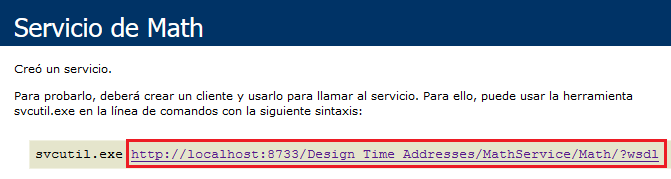
\includegraphics[width=12cm]{URL.png}
	\caption{URL a través de la que obtener el archivo WSDL.}
	\label{fig:URL}
\end{figure}

De esta forma, se generaron en Eclipse las clases necesarias para poder hacer uso del servicio web. Instanciando una de ellas, en cuyo constructor se creaba el \textit{endpoint} que permitía acceder al mismo. Gracias a los métodos existentes en esa clase, fue posible hacer uso de las funciones que determinaban si un número era primo, o resolvían el sistema de ecuaciones.

La parte más complicada al consumar el servicio desde Java, además de la cantidad de información ambigua y/o errónea encontrada en Internet, fue la cantidad de clases generadas a partir del archivo WSDL. Al contrario que con el Visual Studio, que sólo generaba 2, y con un código mucho más sencillo de entender, el generado en Eclipse resultaba de comprensión mucho más difícil. Inicialmente, no teníamos claro como acceder a las funciones necesarias, ya que parecía que se repetían en distintos archivos, y las pruebas iniciales resultaron en errores de todo tipo. Con un poco de investigación, se llegó a la solución aparentemente correcta, instanciando la clase ``IMathProxy'' desde otra clase llamada ``Consumer''. De esta forma, y siguiendo el flujo de ejecución del programa, fue posible acceder a los métodos implementados en el servicio web.


\section{Conclusiones}

La resolución de esta práctico conllevó más tiempo del que, visto una vez hecha, parece necesario. Ambas ampliaciones requirieron bastante investigación y búsquedas en distintas páginas. Además, si bien la primera supuso un problema mucho más directo, el consumo del servicio desde Java era algo que no habíamos estudiado con anterioridad. Por lo tanto, aunque no había más que replicar el funcionamiento conseguido con el Visual Studio, este inconveniente y la aparición de constantes errores dificultó bastante la consecución de un resultado satisfactorio.



\end{document}